\chapter{Introduction}\label{Chap:Intro}
\section{Head 1}
%P1. Eq natural
\lipsum[1]

% \Figure[t!](topskip=0pt, botskip=0pt, midskip=0pt)[width=0.6\textwidth]{img/p-wave.png}
% {P-wave, S-wave, Surface-wave, and PGA\label{fig1}}

\begin{figure}[ht]
    \centering
    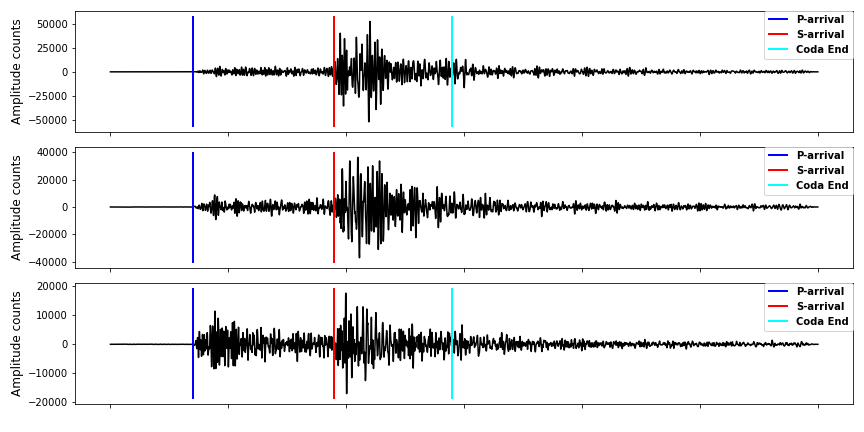
\includegraphics[width=0.9\textwidth]{img/3ch.png}
    \caption{Three channels of seismic wave}
    \label{fig:3-wave}
\end{figure}

\lipsum[2]

\begin{figure}[ht]
    \centering
    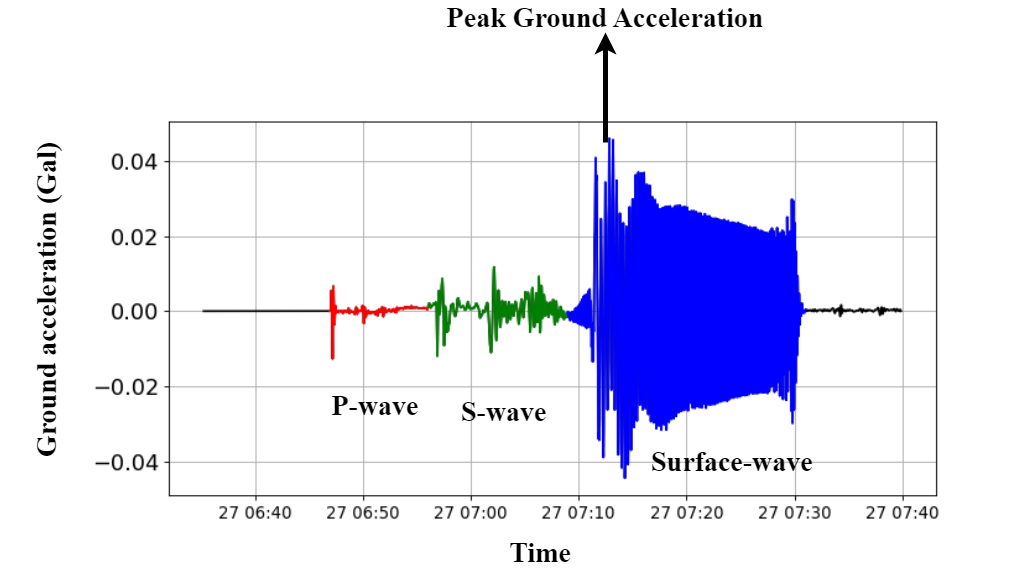
\includegraphics[width=0.9\textwidth]{img/p-wave.png}
    \caption{P-wave, S-wave, Surface-wave, and PGA}
    \label{fig:p-wave}
\end{figure}

This is the figure referenced in \ref{fig:3-wave} and \ref{fig:p-wave}. 

\section{Head 2}
%P2. EEW
This is how to cite the references~\cite{gasparini2007earthquake, allen2019earthquake}.

\lipsum[1]

\section{Head 3}
This is the list:
\begin{enumerate}
    \item Item1.
    \item Item1.
    \item Item1.
\end{enumerate}



\subsection{Sub head}
\lipsum[1]

\subsection{Sub head}
\lipsum[2]

